\chapter{Old Analysis - Experiments and notes}
The two main hypotheses of this thesis are, 
\begin{enumerate}
 \item that the financial sector affects the ownership of housing and the class structure of society, 
    \item that this may have implications for urban productivity. 
\end{enumerate} 
Many parameters in the model will have some effect, but we have to focus on policy-relevant parameters. These a) can be manipulated, and b) can have measurable effects.


\section{Effect of the financial sector on ownership} 
We need to have 
\begin{enumerate}
    \item a set of measurements if ownership

        \begin{enumerate}
        \item number of homes, share of homes by category(owner occ, owner rented), 
        investor rented
        
\begin{tabular}{|r|c|c|c|}\hline
            & owner occ& owner-retired & bank-rented\\ \hline
number      & && \\ \hline
share       & && \\\hline
\end{tabular}

        \item Aggregate Mortgaged share of owner-occupied homes over time 
\[M_t=((1+r)**2-(1+r)**t) / ((1+r)**20-1)\]
\[Share\_mortgaged =\frac{\sum_i M_{,i}}{\sum_iP_{,i}}\]
        \item
        \item
        \end{enumerate} 


I imagine an output like this:

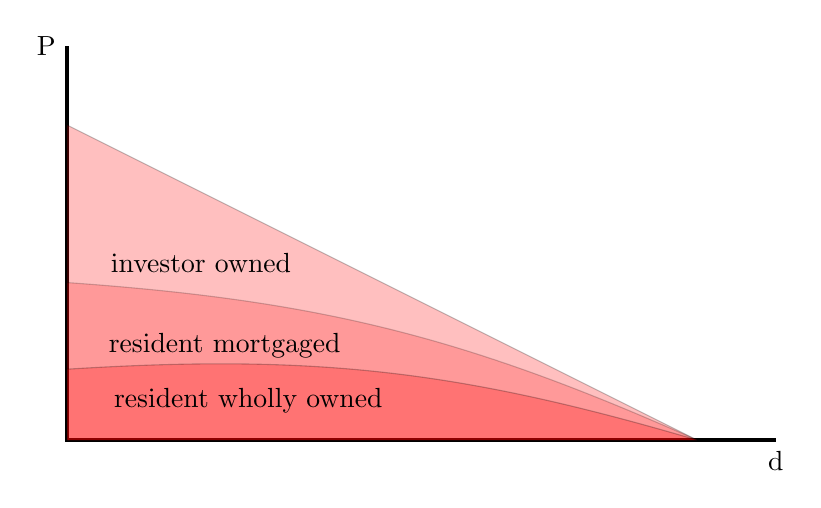
\begin{tikzpicture}
  \draw [ultra thick](0,5)node[left]{P} --(0,0)--(9,0)node[below]{d}; 
  \draw[fill=red, opacity=.25](0,0)--(0,4)--(8,0);  
   \draw[fill=red, opacity=.2](0,0)--(0,2) to [bend left=10](8,0);  
   \draw[fill=red, opacity=.25](0,0)--(0,0.9) to [bend left=10](8,0);
   \node at (2.3,.5)[]{resident wholly owned};
   \node at (2,1.2)[]{resident mortgaged};
   \node at (1.7,2.25)[]{investor owned};
   
\end{tikzpicture}

A similar picture with time on the horizontal axis

    \item parameters of the financial sector  that might affect that structure
    \begin{enumerate}
        \item capital gains tax
        \item interest and mortgage differentials
        \item tightening mortgage limits for owners
        \item transaction cost
        \item density
        
    \end{enumerate}

We can stabilize a city and then make a change to see the effect.

    
\end{enumerate}
\subsection{Results}
These are impressionistic notes from early batch runs.
\begin{itemize}
 \item increasing density range [100, 300, 400, 600]
    \begin{enumerate}
        \item ownership share peaks between 400 and 600. ***
        \item increases mpl
        \item increases firm size
        \item increases fir numbers
        \item decreases peak k
        \item increases city extent
    \end{enumerate}
    
    \item increasing subsistence wage range [30000, 50000, 70000, 90000]
    \begin{enumerate}
        \item decreases ownership share !??. 10 T->100\%  40-> 30\%
        \item seems to reduce mpl
        \item increases firmsize 
        \item Workforce diverges between 50 + and 70 dwn. ***
        \item decreases city extent
        \item increases then decreases firm capital ***
        \item slows growth of workforce

     \item increasing gamma range [0.1, 0.09, 0.08 ]
    \begin{enumerate}
        \item ownership share       
        \item mpl   up              
        \item firm size at up .09 dips and rises   
        \item total workforce up at .09 dips and rises
        \item number of firm number up at .09 dips and rises
        \item k    up peaks at .08                 
        \item city extent    up at .09 dips and rises          
    \end{enumerate}

     \item increasing discount rate.  range [0.1, 0.09, 0.08 ]
    \begin{enumerate}
        \item ownership share  strange sawtooth, generally rising
        \item mpl     no effect              
        \item firm size       no effect         
        \item number of firm number no effect 
        \item k           no effect           
        \item city extent    no effect           
    \end{enumerate}

    
    \item max\_mortgage\_share': [1.0, 0.9, 0.8, 0.7, 0.6]
    \begin{enumerate}
         \item ownership share  strange sawtooth, generally rising
        \item mpl     no effect              
        \item firm size       no effect         
        \item number of firm number no effect 
        \item k           no effect           
        \item city extent    no effect               
    \end{enumerate}


 \item increasing'ability\_to\_carry\_mortgage': [0.35, 0.28, 0.2]
   \begin{enumerate}
         \item ownership share  strange sawtooth, generally rising
        \item mpl     no effect              
        \item firm size       no effect         
        \item number of firm number no effect 
        \item k           no effect           
        \item city extent    no effect  
     \end{enumerate}


      \item increasing 'savings\_rate': [0.5, 0.3, 0.2]
   \begin{enumerate}
         \item ownership share  raises saw tooth
        \item mpl                   no effect
        \item firm size             no effect         
        \item number of firm number no effect 
        \item k                     no effect           
        \item city extent           no effect  
     \end{enumerate}

  
   \begin{enumerate}
         \item ownership share  
        \item mpl            
        \item firm size            
        \item number 
        \item k         
        \item city extent   
     \end{enumerate}
    \end{enumerate}
    


\section{Effect of the financial sector on productivity}
We need to have  
\begin{enumerate}
    \item a set of measurements if ownership
    \item parameters of the financial sector  that might affect that structure

\end{enumerate}

  
\section{Experiments}
  \begin{enumerate}
    \item effect of reducing transport cost $c$
    \item effect of adding a service sector $N_{total} = N(1+z)$ then $N^\gamma \rightarrow  N_{total}^\gamma$
    \item \textbf{effect of adding a service sector whose size depends on the retained income of residents.}
    \item changing density
    \item low-wage immigrants
    \item effect of interest rate spread on housing ownership
    \item 
    \item 
    \item 
    \item 
    \item 
   
    
\end{enumerate} 
    
\end{itemize}
\subsection{What else will affect price and should be included in the regression?}

\newcounter{foo}
\newcommand{\num}{\addtocounter{foo}{1}\thefoo. &}
\newcommand{\Rnum}{\addtocounter{foo}{1}\thefoo. &\vspace{-.3cm}\color{red} }
\section{Variables to track}

\begin{tabular}{lp{8cm}l}
\hline
\num Wage premium  &$\omega$\\
\num workers in a firm &$n$\\
\num workers in a firm &$n$\\
\num output of firm &$y_F=y$\\
\num Firm MPL& $\beta y_F/n$ \\ 
\num  population of workers &$N=F*n$\\
\num total population & $factor * N$\\

\hline
\num number of homeowners &\\
\num number of tenants &\\
\num number of institutional owners &\\
\num number of homeowners who rent&\\
\num number of homeowners with second home&\\


\hline
\num total taxes & $\sum_j t*P_j$ ?\\
\num taxes invested in productivity& $tProdShare * total_taxes$\\
\num taxes invested in Amenities& $tAmenShare * total_taxes$\\

\hline
\Rnum  urban firm-generated surplus &  $(A * N**beta) - (N/n_R * Y_F)$ \\
\num \\

\num total homeowner wealth& $\sum_i(P_I - M_i) + \sum_i S_i$\\
\num homeowner savings invested in productivity & $SProdShare * \sum_i S_i$\\
\num total city output& $Y=F*y$\\
\num  Total Factor Productivity (TFP)& $\frac{Y}{rk+(\omega+psi)N}$\\
\num external investment & $\sum_f K_F$\\
\hline
\end{tabular}

\begin{tabular}{lp{8cm}l}
     &  \\
     &   \\
\num expected rate of price increase over T& $\dot P^e_\mathbb{T} = \left(\frac{\frac{1}{r}\die{\omega}{t} }{P_T}\right)^T $ \\
\num total rent on property& $N(\omega +\mathbb{A}^{net})$ \\
\num total urban locational rent& $\pi(\omega +\mathbb{A}^{net})^2/3c$ \\
\num dissipated rent &$\sum_i^N c_id_i$ \\ 
\num available rent. & $\sum_i^N(\omega -cd +\mathbb{A}^{net})$\\
\num Mortgage interest captured by the finance sector& $MortI=\sum_i r_iM_i^{balance}$ \\
\num Total rent captured by the finance sector& $FinRent = MortI + \sum_j R_{N, j}$)\\
\num share of city-owned by finance& $\sum_i^N M_{i,t} +$ value of property ???\\

\num locational surplus   &  $Surp = \sum_j (/omega- c*d) $\\
\num financial share of surplus & $FinSurpShare = FinRent / Surp$\\
%\num  Amenity & $\mathbb{A}^{net}$\\ 
    %fixed. We want total amenity including utility
\num financial share of city & $FinCityShare = \sum_i^N M_{i,t}$ \\
   %two parts  separately -- (pop with density and seed) * omega
\num GDP Growth &$N(\omega +\mathbb{A}^{net}) + r F(k^U-k^R)$.\\
            &(not a rate) ($(k^U-K^R)=\Delta k$)\\
  \end{tabular} 

 Additional items 
\begin{enumerate}  
\item Total Rent captured by the finance sector is the sum of the interest collected on all mortgages ($\sum_i r_iM_i^{balance}$), where $j$ indexes households,) plus the \textbf{net} rent on rented housing ($+ \sum_j R_{N, j}$), where $j$ indexes properties (Just those owned by the bank Those not owned by the bank represent extractions by small landlords. The Financialization study had a name for this class.).

\item Rent captured by the finance sector divided by urban surplus is the share of surplus captured by the financial sector






\item Output of a  typical rural firm, Equation~\ref{eqn_Rural_output} 
\[Y_R=\frac{n_R*\psi}{\beta_F}\]

The output of a rural firm is a constant  providing a reference line for the output of the urban firms. %calculated in appendix 2 to get initial values

  \item excess profit: all profit is excess because the cost of capital has been covered.
    \[\Pi^{excess}=F*(y_{U,t} - r*k -)(\omega+\psi)n_{U, t}\]

 \[RB = M_0 * (((1 + r)^20) – ((1 + r)^p)) / (((1 + r)^n) – 1)\]

Where:

    P = principal amount of the loan (\$10,000 in this case)
    
    r = monthly interest rate (r=r\_prime + margin)
    
    n = total number of payments 20 years, one per year
    
    p = number of payments made so far (12 in this case)   

\end{enumerate}



 \subsection{for the price model}
% make sure the regression model makes sense. price should fall with distance by the present value of the cost of transportation: $cd/r$. Only $d$ varies across properties. In a regression for price the beta for distance should be $c/r$. This can serve as a check  

% We can think of properties at the same distance as a "transportation-equivalent neighbourhood'' such that 
% \[d_j=d_k,\]
% where $d$ is distance.  (or $\omega-cd_j=\omega-cd_k$.  We expect prices to behave the same in these neighbourhoods. You can add dummies for other neighbourhoods to the model later if you add neighbourhood features or specific amenities. 

% In the regression you just add $d_j$

\subsection{Estimation P-dot from the model }
% The higher the rate of price increase the more people will want to buy or hold the property. 

% In the regression you just  $\dot P_{t,j}$

% By definition, $\dot P_{t,j}$ is \[\dot P_{t,j} =\frac{P_{t,j}-P_{t-1,j}}{P_{t-1,j}}\] for each property. This can be calculated property by property. What if there are very few properties that have changed hands  in the last two periods? 


% Will it serve as as plausible value for $\dot P_{t,j}$? Yes.

% The average of this value across the neighbourhood is the average neighbourhood price growth. It WILL vary by distance. To see this consider a rise in $\omega$ and two properties, one at the centre and at the edge of the city. The one at the centre has a price $(\omega + a\psi)/r$ and the edge property  has a price $(a\psi)/r$ Both increase in value by $\Delta\omega/r$, so the rate of price growth must differ.



\subsection{r-code to graph remaining}
The figure below illustrates the path of Mortgage remaining, which we need for certain wealth calculations (if an owner wants to get a second mortgage.
)
% n<-240]%
% r<-.05/12
% t<-seq(0,240,1)
% rm<- ((1+r)^n-(1+r)^t) / ((1+r)^n-1)
% plot( rm) 
In Python 

\[M_t=((1+r)**2-(1+r)**t) / ((1+r)**20-1)\]

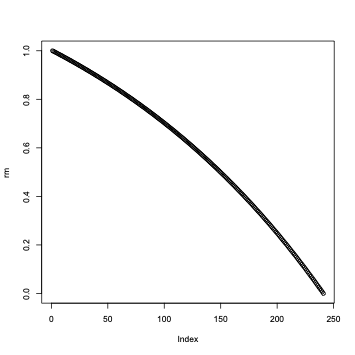
\includegraphics[scale=.25]{fig/declining-balance.png}
  
    


\section{Main}

% Get banks 'We are the biggest innovators in history quote'
%``Financial engineering has created a rentier class, a modern feudal system, and the biggest beneficiaries of all that extra debt have been the bankers.'' Times, Sunday Times (2016) 


% Repeat from introduction contributions
% Note multiple drivers - 
NOTE \textbf{not sensitive to any advantage being true all of the time. etc } IN THE STRUCTURE.
% can be thought of as regimes containing tipping points, the feduciary duty of governance is to sustain the regimes society chooses, to make that process of choosing tractibel labs, Kahane.

% MAIN PLOTS DIRECT ANALYSIS
% RESILIENCE ANALYSIS 
% DISCUSSION AND EXTENSIONS

In the base model, we only allow the radius of the city to change, and not the density and firm hiring behaviour.\footnote{Complex city form, density patterns, and alternative hiring patterns, can be easily incorporated in the computation model. We expect that they would not significantly affect our conclusions.}  
% model rules, and individual 
%and the job search process. 
% In practice, many other factors impinge on these choices. %additional decision factors, agents, driving variable, and \gls{stochastic} elements enter the model. 

{\color{red}


\section{System dynamics}\label{sec_model_dynamics}
Combined, the three submodels we have just described make up a complex system with different types of agents interacting over time. It is an \gls{open system} that is growing, with financial and population flows in and out of the system. We have simplified, assuming that there is a competitive market for output driving urban productivity. There are two main \glspl{feedback loop}: the productivity-wage, population-productivity loop that we call the Alonso-Jacobs cycle, and the speculative investment-price, inflation-investment cycle that may produce price bubbles. 

A system of this sort inevitably has distinct dynamics that can, depending on \glspl{critical parameter}, produce surprising and even counter-intuitive results.  Whether this system is dynamically stable is not clear at this point. It may converge to an equilibrium population or not, and it may or may not exhibit cycles or even chaotic behaviour. We have tried to simplify as much as possible precisely because we are interested in the dynamics of the system

System behaviour depends on the speed with which system stocks adjust. In principle the behaviour of the system may be very sensitive to specific parameter values. We know that certain variables , like ownership  shares are bounded between zero and one although the housing stock itself is variable.  

We have not introduced  stochastic elements into the core model on the grounds that it is easy to add noise, but hard to understand its effect unless you have a baseline to  compare it to.

One advantage of beginning with an agent-based model is that we are not imposing linearity, or a-priori distributions on the behaviour of agents. These assumptions might make the model more tractable, but they have little empirical or theoretical justification.

It should be obvious that Figure~\ref{fig-flow-full-model} leaves out many links and potential links. For example, worker buyers and investment buyers have correlated costs of capital. The strength of the correlation may matter. Population size or composition may affect amenity - which we have not models---and the amenity levels may then affect the population response. The amenity link may feed into the bidding for homes, which may then affect the population mix. Our modelling strategy has been to think a lot about such cross-links and extensions, and then to leave them out until we can add them to a well-understood and even teachable model.
}

\section{Financialization: implications of  population or productivity growth}

Our model is a dynamic  one, concerned with growth and financialization. We have described the components separately and  generally described them in static terms. Rent theory in  particular was a static described as though rents never changed. With a small addition to the figure from Chapter~\ref{chapter-space}, however, we can begin to explore the effects of rising population or productivity. 

In Chapter~\ref{chapter-space} we limited our discussion to what is termed differential land rent, which results from differing transportation costs. It is the key concept in the Alonzo model. The city grows until adding more land at the edge of the city generates no land rent because the value of access to the city centre is eaten up by transportation costs. If the population or productivity increases   drive up the the value of access, the price of land  will rise across the entire city. The higher land value would eventually lead to an expansion of the housing stock, moving the city edge in Figure~\ref{fig:absoluite_rent} outward. The differential rent would expand as well.

If we focus on the increase in rent before the housing stock can expand, which we show as the orange rectangle in Figure~\ref{fig:absoluite_rent}, it is clear that increased productivity is translated into increased rent on existing properties.\footnote{The orange rectangle corresponds in this setting to what Marx called ``absolute rent'' \cite{dasilvaAbsoluteRent2018}. } The orange rectangle represents value of the increase in the wage across the entire city. When the stream of rent it is discounted to the present it represents \textbf{the total increase in land value across the entire city}. 

Like Marshall's quasi-rent, This rise in rent provides an incentive to expand the stock of productive housing capital.  It does not disappear  as a quasi-rent would, however. Instead it appears as a windfall gain for owners. In our analysis it has another effect: it will attract speculative purchases of the existing housing stock. It is one of the drivers of the financialization of the housing stock. 


\begin{figure}
    \centering
    
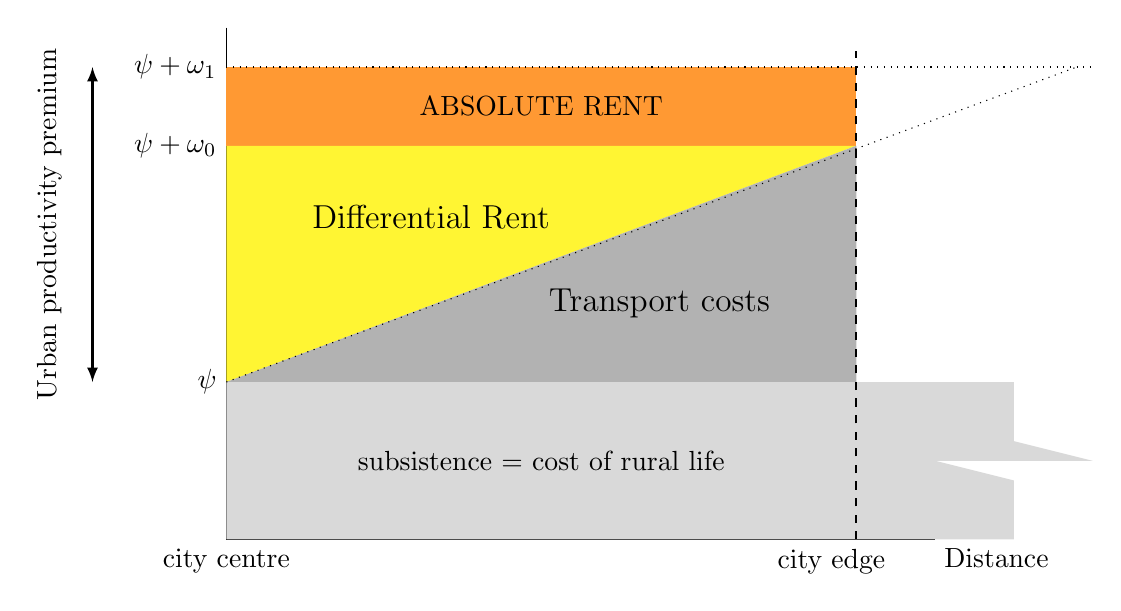
\begin{tikzpicture}[domain=0:2]
%\draw[thick,color=gray,step=.5cm, dashed] (-0.5,-.5) grid (12,5);

\draw[line width=.01 ] (1,6.5) -- (1,0)node  [below] {city centre}--(10,0) node[below right] {Distance};
%\draw[line width=.01, green ] (0,0) -- (10,0) node[right ] {Distance};
\node[below,text width=2cm]at (9,0) {city edge};

\fill [orange!80]  (1,5) --(1,6)--(9,6) --(9,5)--cycle;
\fill [yellow!80]  	(1,2) --(9,5)--(1,5) --cycle;
\fill [gray!60] 	(9,5) --(1,2)--(9,2) --cycle;
\fill [gray!30] 	(1,0) --(1,2)--(11,2) --(11,1.25)-- (12,1)-- (10,1)--(11,.75)--(11,0)--cycle;



\node	at 	(1,5)[left]{$\psi +\omega_0$} ;
\node	at 	(1,6)[left]{$\psi +\omega_1$} ;
\node	at 	(1,2)[left]{$\psi$} ;

\draw[thick , dashed] (9,0)  -- (9,6.2); 
\draw[dotted] (1,6)  -- (12,6); 
\draw[dotted] (1,2)  -- (11.8,6); 

%\draw[thick,color=red] (1.5,0) -- (1.5,1) node[below right] {Fixed cost} -- (1.5,1.5) --(10,3.25)node[above left] {total cost};

\node at (5,5.5)[] 	{ABSOLUTE RENT} ;
\node  at (6.5,3)	{\large Transport costs};
\node  at (3.6,4.1)	{\large  Differential Rent};
\node at (5,1)[] {subsistence = cost of rural life} ;
\node at (-1.25,4)[rotate=90] {Urban productivity premium} ;
\draw[thick,latex-latex] (-.7,2) -- (-.7,6) ;
\end{tikzpicture} 

    \caption{Growing productivity, population, and rent. Rising productivity and/or population will increase rents. With slow or no increase in density or area,  absolute rent grows and becomes a target for financial capital.  }
    \label{fig:absoluite_rent}
\end{figure}

\subsection {Productivity growth}
In this case, the orange rectangle in Figure~\ref{fig:absoluite_rent} shows the effect of an increase in the wage premium from $\omega_0$ to $\omega_1$. We can assume that the wage has been raised by firms in order to attract more workers because productivity has risen. An increase of this sort in our model may hae resulted  from past population growth generating additional agglomeration effects. Since such effects accumulate slowly, the figure illustrates an increase due to previous population growth that gradually brought improved methods and machinery, new products or even new markets. The    
The housing stock has not yet adjusted.  Any fraction of the increase in productivity  flowing into profits does not appear in the figure. 


Initially the increase in the wage would appear as increased saving and consumption for resident workers. For tenants, the improvement would be temporary. Landlords would realize that tenants could pay higher rent or new tenants would bid more for housing. The result is that non-resident owners would eventually extract part of  the increase in productivity. That fraction would grow as the financialization of the housing stock proceeded expanded 

In time the city would expand to provide new housing. The expansion would proceed until the diagonal line extended to the height $\phi+\omega_1$.\footnote{The figure only allows for increasing area and not increasing density.}  

Of interest here is that, at the moment represented by the figure, a significant rise in land rent across the entire city is in the future and therefore increasing house prices are predictable. Agents that foresee the capital gain would invest. The pool of new workers who can afford to purchase might be small, however, while the pool of available financial capital would be large. It is reasonable to expect that the increase in urban productivity would tend to drive increased financialization of the housing market.

In this situation there is a possibility that real estate investment might squeeze out productive investment. Finance would flow to expanding the housing stock, which is productive investment.  Would financial capital flow into investment in city firms or into speculative investment in existing housing? Real estate investment might  draw capital away from productive investment. A great deal might depend on assessments of the riskiness of the different investment channels.

\subsection{Population growth}
Population growth will operate on the same variables  but in a different way. There is a debate about whether urbanization drives  growth or growth drives urbanization. We observe in-migration as one apparently independent driver of urban population growth,  so it makes sense to examine the effect of an externally driven increase in urban population. 

Increased competition for housing will drive up rents and prices. The increase in rents will not affect owner-occupiers directly, although they might see and increase in boomerang children or an increase in opportunities to rent out part of a home. Both of these effects would tend to increase home values for owners, make them less likely put a home on the market. 

The increase in rents will affect tenants and in-migrants. It may eat into their consumption or savings. It will also drive some low-pay workers out of the city and increase wage demands. Wages will have to rise, probably reducing profit and investment in the city. The rising rents will have the tendency to increase financialization of the housing stock as in the previous subsection.


\section{The larger setting of this analysis for Canada}

\subsection{Rent extraction}

This thesis demonstrates the very basic principle of increasing urban rent extraction through the financialization of the housing market. 
{\color{red}(One of my key research findings/methods/outcomes in recent years.)}
 
The institutional basis is the ownership structure that allows the social surplus generated by agglomeration to be privately appropriated. Even in the recent past, this process contributed to the development of a home-owning middle class and to widely distributed wealth. Financialization is now narrowing the distribution of wealth and shrinking the equity-owning middle class. {\color{red}(One of my key research findings/methods/outcomes in recent years.)}

Taken together the two points above describe  one of the deep causes of the current and continuing housing crisis.

It is our contention that the process we describe will also undermine the productivity of cities and the quality of urban life. {\color{red}(The most pressing incomplete research issues of my research to date.)} 

% \documentclass[tikz,minimum size=20cm]{standalone}
% \usepackage{tikz}
% Four Themes for  housing research April 21

% \usetikzlibrary{shadings, shadows, shapes, arrows, calc, positioning, shapes.geometric}
% \usepackage{pgfplots}
% \pgfplotsset{compat=1.16}
% \usepackage{mathtools,amssymb}
% %\input{Preamble}
% %\input{(SpecialDistanceCourse}
% %\input{FRAMES}
% \begin{document} 
 
 \begin{tikzpicture}%[scale=.8]
    \tikzstyle{every node}=[font=\small]
%\draw[help lines,step=.5] (0,-11) grid (11,11);

%  LOCATION OF ALL NODES
\coordinate (Extraction) at (0,3);%PREFACE
\coordinate (Tenure) at (5,3);%
 \coordinate (Corridor) at (5,0); %history
\coordinate (Lifeboat) at (0,0); %
%\coordinate (d) at (9,9);%


%.  CIRCLE NODES
% \fill[red, fill opacity=.8] (0,0) circle (4cm);
%\fill [gray, fill opacity=0.2] (m) node [text width=2cm, black, opacity=1] 				(community)	{} circle (3cm);
%\fill [gray, fill opacity=0.1] (oo)  node [text width=2cm, align=left, black, opacity=1] 		(econ) {} circle (3.5cm);
% \node at (e) [ ] 		(comLtabel) {Data};
% \node at (g) [ ] 		(ecLabel) {THEORY};
	
%\node [circle, draw,  fill=gray, opacity=.5,, text width=1.5cm] at			 (aa) 		(preface)		{HYPOTHESIS};
%\node [] at			 (f) 		(plan)		{\Huge PLAN};
			%\draw [fill=blue, fill opacity=0.35] (b)node [text width=2cm, align=center, black, opacity=1] 			(history){History: New is Old} circle (1.2cm);

\node[fill=red!30, regular polygon, regular polygon sides=6, draw, align=center]at (Extraction) (ExtractionP) 	{\color{black}Rent  \&\\Finance};%Extraction \\and \\Financialization} ;

\node[fill=yellow!30, regular polygon, regular polygon sides=6, draw, align=center] at (Tenure) (TenureP) {Tenure\\ and\\ Wealth} ;

\node[regular polygon, regular polygon sides=6, draw, align=center] at (Corridor) (CorridorP)	{Socal\\ Wealth \\Corridor};

\node[fill=green!30, regular polygon, regular polygon sides=6, draw, align=center] at (Lifeboat) (LifeboatP)	 {Lifeboat\\Canada};

% LINKS
%\draw (J) node [text width=6cm, text centered] {Economic Development };
%\draw ()--();
\draw [gray, line width=2mm,-> ](ExtractionP)to [bend left=35](TenureP);
\draw  [gray, line width=2mm,->](TenureP)to [bend left=60](CorridorP);
\draw  [gray, line width=2mm,-> ](CorridorP)to [bend left=35](LifeboatP);
\draw  [gray, line width=2mm,-> ](LifeboatP)to [bend left=60](ExtractionP);

% \draw [gray, line width=2mm,-> ](whatis)--(joint);
% \draw [gray, line width=1mm,-> ](joint) to [bend right=25](efficiency);
% \draw  [gray, line width=1mm,-> ] (joint) to [bend left=20](capital);
% \draw [gray, line width=1mm,-> ](joint) to [bend right=20](externalities);
% \draw [gray, line width=1mm,-> ](joint) to [bend left=25](trans);
% \draw  [gray, line width=1mm,-> ](joint)->(pubgoods);
% \draw  [gray, line width=.5mm,-> ](capital) to[bend left=25](small);
% \draw  [gray, line width=.5mm,-> ,dashed](joint) to[bend left=7](forestryEC);
\end{tikzpicture} 

% \end{document}

\subsection{Tenure}
The three points above make  it clear that developing \textbf{tenure structures} that stop or reverse the two big trends we highlight above are part of any durable solution to the housing crises. The productivity of our communities has to be maintained with some form of social equity if the wealth creation of the community is not to be sucked away.     {\color{red}(Research in financing and tenure structures, as well as regulatory support and the social innovations required appears is necessary to lay the groundwork for any robust response to the current housing crisis. It will take  multidisciplinary collaboration  \dots}

\subsection{Community wealth corridors: the Oasis model}
More than half of Canada's population lives within  one hundred kilometers of a line from Windsor to Quebec City. More than half of Canada;'s immigrants come to that strip. Canada is now crawling toward a high-speed rail system in that strip. It is crucial to understand that more than half of the housing that will be built in Canada in the next 30 years will be on that corridor. 

It could be a social and environmental disaster. Or we could be building enormous social wealth for the most environmentally integrated society in the  world. 
    
        {\color{red}(My vision for housing research in Canada?would focus on creating a social wealth corridor in which the housing assets are owned by the people, not outside capital, and the communities are genuinely sustainable. This will take not just building design, but integrated building systems, linked to the evolving transportation system and )}

 \subsection{Lifeboat Canada}
 All of these issues are nested inside a broader set of challenges: climate migration. To protect Canadians it will be necessary for Canada to make its economy and its cities more resilient, carbon free  increasingly self-sufficient while expanding the housing supply and  maintaining the quality of life and of the local environments. 
 
 At the same time, it is very likely that Canada will be pressed to, and will want to, take in a fair share of the climate refugees expected from  other parts of the world this.

 I think about this  set of challenges as the ``Lifeboat Canada'' challenge. We have to be able to stay afloat while rescuing as many as we can. Lifeboat Canada presents a massive design problem  for our  existing cities, for the many linked centers related to cities, for the transportation system and for environmental design. 

 It takes us back to how we can capture and use the social wealth that create to survive the coming storm. 
 

  {\color{red}(One part of my vision for housing research in Canada  is to start planning for ``Lifeboat Canada''that proofices XXX (topics, goals, methods for knowledge transfer, collaboration structures, etc.)}
 
\section{Financialization: implications of the bidding rule}

There are some implications of the financialization mechanism:
\begin{enumerate}
\item A large $m$ magnifies the return. (The downpayment is smaller as a fraction of the price, increasing the investor's leverage). 
Given the  common rule that mortgage payments cannot exceed some fraction of disposable income, the wealthy will be able to borrow larger amounts and at lower interest rates than the less wealthy. At any distance from the centre they will be able to make a higher bid.

\item A lower mortgage interest rate increases the return by lowering interest payments. The cost of capital is known to differ for rich and poor.  The wealthy can generally borrow  at lower interest rates than the less wealthy. 

\item A lower discount rate $\delta$ reduces the subjective rate of return.  Poverty in assets and cash liquidity constraints are correlated with higher rates of time preference  \cite{carvalhoPovertyTimePreference2010}\cite{holdenPovertyMarketImperfections1998}. If agents discount at their borrowing rate, wealthier agents may have a lower subjective rate of time preference and therefore value properties more highly. 

\item Higher expected price appreciation increases the attractiveness of an investment. Financial corporations and the wealthy are likely to have better price forecasts than  the occasional home buyer.

\item Higher rents make the unit more profitable. Higher expected  rents may result from expecting greater price appreciation  leading to raising rents for tenants. Lower discount rates may give future rent increases greater present value.

\item Lower maintenance costs increase profits. There may be scale economies in the maintenance  of rented housing. 

\item Lower tax rates decrease holding costs and increase the value of the investment. There may be opportunities to shelter income with land held for investment (speculative) purposes. Tax treatment of income and capital gains as well as interest deductibility may also provide advantages for institutional buyers and investors.%\footnote{Case and Schiller \cite{LOST_CaseandSchiller} observe that (source?) `` \dots increases in real per capita income all are positively related to excess returns or price changes over the subsequent year.''} 
\end{enumerate}

Some  of these conditions (1-3) hold generally for wealthier actors. Others (4-7) may be available only to institutional investors.  Financial corporations in particular may have advantages relative to individual investors, making it reasonable to expect that financial corporations increasingly dominate urban land 
markets.\footnote{Fr\'ed\'erick Demers \cite{demersModellingForecastingHousing2005} found that the response of housing investment to interest rates has become more pronounced over time. This suggests a rising share of financial investors relative to buyers focused on housing services. Case and Schiller \cite{caseThereBubbleHousing2003} observe that `` \dots increases in real per capita income all are positively related to excess returns or price changes over the subsequent year.''}  

Since interest rates are lower for those with higher wealth, the analysis implies, consistent with the empirical evidence, that net returns for investment are increasing with wealth. Large wealth holders will get higher expected and actual rates of return on land than those with lower wealth holdings. Managers of large pools of capital will have an even greater   advantage. Overall, Equation~\ref{eqn-bid-price} implies  sales generally go to the richest participant.
 
%  \footnote{Case and Schiller \cite{LOST_CaseandSchiller} observe that (source?) 
%  `` \dots increases in real per capita income all are positively related to excess returns or price changes over the subsequent year.''} 

% The conclusion that we draw from the analysis above is that  financialization of urban housing benefits a rentier class of urban landholders. There is evidence that it benefits a globally distributed class of rentiers.  



\section{Financialization as system change} \label{section-system}
We established that, at least in theory,  financial institutions and the wealthy are likely to own increasing shares of the housing stock. the theoretical conclusions is consistent with what has already happened in the Canadian Housing market. Recent data from Statistics Canada \cite{fontaineResidentialRealEstate2023} suggests people who own more than one property in Ontario make up more than 25\% of buyers in the province. (The proportion of investors among owners varied from 20.2\% in Ontario to 31.5\% in Nova Scotia.)
Just under one in five properties overall was used as an investment.
In Ontario 41.9\% of condominium apartments are investment properties \cite{statisticscanadaBuyRentHousing2022}.

The immediate social implications are fairly obvious. As Statistics Canada points out, these trends might limit the number of properties available to buyers who intend to use it as a primary place of residence  \cite{fontaineResidentialRealEstate2023}. Statistics Canada reports that latest census release, two-thirds of Canadians owned a home in 2021, down from a peak of 69 per cent a decade earlier. The decline is was higher for younger members of the population. 

When the homeownership rate goes down, the rental rate goes up. The 2021 Canadian Housing Survey reported that the number of renter households increased  at over twice the pace of owner households, pushing down the homeownership rate in Canada. If the trends continue, Urban Canada will gradually change from a society dominated by homeowners to a predominantly tenant society. Since wealthier buyers are advantaged in the market, the younger and poorer parts of the community will be increasingly excluded from ownership. Financialization will increase income and asset inequality in cities.

Combined with rising housing prices the effect will be to squeeze lower-wage households closer to what we have termed to subsistence level and make it harder for low-wage workers to live in the city. The city requires low-wage workers for many of the services, so labour shortages are a possibility. Labour shortages will squeeze some activities out of the city and are likely to reduce productivity. Labour shortages may push up wages, but in rental markets, landlords can capture much of any increase in wages. 

The incentive structure in our model was derived purely from the point of view of an individual investor. Examination shows that investment incentives favour the wealthy and institutional buyers, but that does not necessarily imply that the process of financialization will drive social transformations. Individual choices are at most  a link in the chain. Modelling  allows us to identify which parameters are most influential. 

A question that is especially important is whether the process of financialization and tenentization our micro model suggests is reversible:  high levels of home ownership we have seen throughout the 20$^{th}$ century, as Purdy \cite{purdyPropertyOwningDemocracyHome1993} suggests, may be ``a transitory phenomenon of the 20th century.''

% .#https://www.jstor.org/stable/j.ctt80wdt Housing the North American City
% MICHAEL DOUCET
% JOHN WEAVER
% Copyright Date: 1991
% Published by: McGill-Queen's University Press
% Pages: 608
% https://www.jstor.org/stable/j.ctt80wdt

 %how financialization might affect  the housing market as a system and some consequences for society in general. At that point we can introduce our specific hypotheses and how we intend to test them.
%***E IF YOU WANT TO INTRODUCE ANEW USE OF THE TERM, CONTEXTUALIZE IN TERMS OF HOW YOU ARE USING THE WORD. IS THIS AN EXTENSION OF HOW YOU USE IT? THIS SEEMS RELATED TO THE MACRO VERSION YOU MENTION ABOVE. MAKE THE RELATIONSHIP CLEAR. I ALSO WONDER IF THIS WOULD BE USEFUL TO MOVE UP. IT FEELS LIKE IT MAKE BELONG WITH THE BROADER CONTEXT AT TEH BEGINNING OF THE CHAPTER? GOOD IDEA I will try it

*e tHIS IS CLEAR BUT COULD BE HELPED BY RESTATING HOW THEY MOVE IT ONTO FINANCIAL MARKETS. JUST A QUICK SUMMARY STATEMENT OF HOW THEY ARE FINACIALIZATION. %EVEN JUST something like \dots They put the ownership of housing onto financial markets. just to keep us oriented in what we are talkign about.

*E I FEEL LIKE THERE IS SOMETHING MISSING BETWEEN THESE TWO PARGRAPHS. %PERHAPS JUST FLESHING OUT WHAT FINANCIALIZATION LOOKS LIKE TECHNICALLY. MAYBE ALSO INSTRODUCE POSIBLE EFFECTS \dots LIKE EVEN JUST INTRODUCE THEM AS QUESTIONS? IT'S BEEN SUGGESTED OR SHOWN THAT ITS CONTRIBUTING TO THE HOUSING CRISIS. tHIS WOULD ALSO BE A GOOD PLACE TO EXAPLIN WHAT YOU MEAN BY ``aS SYSTEMS CHANGE \dots BECAUSE i THINK THAT IS A BIG PART OF WHY YOU SAY NEXT THAT IT NEEDS TO BE UNDERSTOOD \dots BECAUSE IT HAS SUC BROAD EFFECTS

We need to understand the economics of financialization.
% \section{Literature on theory and evidence} % PROVIDE EVIDENCE 	mention theories?
There is substantial evidence that the financialization of urban housing is underway in Canadian cities..

Two questions arise when we observe the growing participation of global capital in the urban housing system: 
\begin{enumerate}
\item How far will the financialization of urban land go? 
\item That are the implications for the urban economy and the welfare of the urban population? 
\end{enumerate}

We can demonstrate that in the absence of policy interventions, differential access to finance capital ensures that capital owners acquire an increasing share of urban land % over time
and therefore capture the growing land rents from urban productivity growth. 

With this insight, growing wealth inequality emerges within a simple, widely accepted model of the urban land market. In the limit, urban residents are tenants, and new residents without capital no longer receive any of the increases in rents arising from the growing productivity of the city. 

%The first question, therefore, is reduced to which capital holders will increase their share of urban land and whether there is any reason to expect the process of financialization process to stop or reverse itself.

% \section{The incentives for financialization}
%Instead, drawing on the ideas of Jane Jacobs, Lucas proposes the city as the unit of analysis. Lucas, Robert (1990), ``Why Doesn't Capital Flow from Rich to Poor Countries?,'' American Economic Review Papers and Proceedings v. 80, no. 2 (May) pp. 92-96.  
%Jacobs, Jane  (1969), The Economy of Cities (New York: Random House).  
% The Death and Life of Great American Cities \cite{jacobsDeathLifeGreat1961}

MOVE The mortgage share and interest rate are functions of the agents wealth %Both the  share of the price  that can be mortgaged, $m$, and the interest rate and the interest rate paid, $r$, are functions of the agent's wealth. 
The discounting factor may be correlated with wealth as well. 

%%%%%%%%  VVVVVVVVVVVVVVVVVVVVVVV   This section May 18 to cut?  V
%%%%%%%%  ^^^^^^^^^^^^^^^^^^^^^^^   This section May 18 to cut?  V
% TODO - add interest rate discussion - (borrowing rates drive land prices up, even if there is no development or improvements, simply because it makes it worth a larger--the effect of low rates, especially for institutional actors have driven a large effect)
%\begin{enumerate}
%
%\item  the buyer and seller calculate the value of the property  differently. 
%
%\item  the  buyer and seller may have different expectations of the path of prices and therefore the stream of rents.
%%There are two standard ways that expectations are modeled
%%	\begin{enumerate}
%%	\item \textbf{Adaptive expectations.} Expectations are largely based on what has happened in the past. 
%%	Under normal conditions most people  have relatively weak incentive to get forecasts about inflation correct and lack the resources and time to purchase expert advice. 
%%	Recent price trends are easily available and likely to be the main source of  information.
%%	\item     \textbf{Rational expectations.} Expectations are based on a model of the future economy. 
%%International investors and banks employ economists and other experts to  forecast prices, exchange rates, and trends in the economy.
%%	\end{enumerate} 
%\end{enumerate}
% Why would  discount rates differ between identical workers? Buyers and sellers are not identical in wealth, . 
%%We could implement the first  explanation either by generating expectational errors based on functional class or wealth. 


\section{Distributional consequences of the analysis}
The analysis in this dissertation makes clear that in addition to distributional consequences, the housing crisis has productivity impacts. Specifically, the analysis in this thesis concludes that, given the ongoing financialization of the housing market:

\begin{enumerate}
\item the financial system will eventually extract all net urban land rents through investment in urban property
\item housing accessibility will become increasingly challenging for disadvantaged groups
\item housing will be largely eliminated as a saving mechanism and asset fr middle income Canadians,  resulting in a systematic decline in the `middle class'
\item that the quality of urban life will decline
\item the economic growth and development of cities is threatened by this financialization
\end{enumerate}


\section{Model dynamics}
How quickly various the housing stock, the population and the rate of rent extraction adjust are key parameters determining the dynamics of the system. We have parameterized each in a simple way in order to conduct sensitivity analysis